\documentclass{beamer}
\usepackage[utf8x]{inputenc}
\usepackage[T2A]{fontenc}
\usepackage[english,russian]{babel}

\usetheme{mybeamer}


\title{Влияние точности входных параметров моделей ядерных реакций на предсказанные выходы $r$-процесса}
\subtitle{Магистерская диссертация}
\author{Негребецкий В.В.}
\institute{МГУ им. М.В. Ломоносова, физический факультет,\\
кафедра общей ядерной физики\\
\vspace{1em}
\textnormal{Научный руководитель: к.ф.-м.н. Стопани К.А.}
}
\date{}

\begin{document}
  \frame[noframenumbering] {
    \titlepage
  }
  
  \frame{
    \frametitle{Распространенности ядер в Солнечной системе}
    \small
    Проблема нуклеосинтеза тяжелых изотопов:
    \begin{itemize}
      \item Легкие изотопы образуются в реакциях звездного горения.
      \item Синтез ядер тяжелее железа энергетически невыгоден.
      \item Таких ядер действительно довольно мало. 
    \end{itemize}
    \center
    \includegraphics[width=\textwidth]{../pics/lodders.pdf}
    \footnotesize
    По данным \textit{Lodders 2003}.
  }

  \frame{
    \frametitle{Механизм нейтронного захвата}
    \small
    Синтез тяжелых ядер в основном обеспечивают $s$- и $r$-процесс.
    \begin{centering}
    \includegraphics[width=0.9\textwidth]{../pics/tracks.pdf}
    \end{centering}
    
    \begin{block}{\bf \small Особенности $r$-процесса}
      \small
      Экстремальные астрофизические условия и участие \textbf{сильно нейтроноизбыточных} ядер.
    \end{block}
  }

  \frame{
    \frametitle{Моделирование нуклеосинтеза}
    \small
    Система уравнений нуклеосинтеза: 
    \begin{equation*}
    \displaystyle 
    \frac{d y_i}{d t} = \sum_{k \in K_i} \pm {\color{blue}\lambda_k} \prod_{l \in L_k} y_l
    \end{equation*}
    
    Особенности задачи:
    \begin{itemize}
      \item Огромная размерность ($\sim 7800$ изотопов и $\sim 10^5$ реакций)
      \item Сверхжесткость системы уравнений 
      \item Неопределенность астрофизических параметров
      \item Недостаток данных о задействованных экзотических ядрах, \\
        \textbf{их характеристики приходится получать из моделей}
    \end{itemize}
  
    \begin{block}{\bf \small Ядерные данные}
      \small
      Влияют на моделирование $r$-процесса через величины астрофизических 
      \textbf{скоростей реакций $\color{blue}\lambda_k$}.
    \end{block}
  }

  \frame{
    \frametitle{Астрофизические скорости реакций}
    \small
    \textbf{Скорость реакции $\color{blue}\lambda_k$} --- это вероятность протекания реакции на единицу времени на единицу концентрации каждой исходной частицы.
    
    \begin{equation*}
      \displaystyle
      \lambda(T) = \int_0^\infty \sigma(E) \rho(E, T) dE,
    \end{equation*}
    где $\rho(E, T)$ --- энергетическое распределение.
    
    \vspace{0.5cm}

    \begin{itemize}
      \item Для $r$-процесса $\sigma(E)$ можно получить лишь из теоретических моделей (статистический подход Хаузера--Фешбаха).
      \item Для этого нужно характеристики нейтроноизбыточных ядер (например, массы), которые \textbf{тоже получают из моделей}.
    \end{itemize}
    
    \begin{block}{\bf \small Влияние ядерных моделей на моделирование $r$-процесса}
      \small
      Можно проанализировать, \textbf{варьируя массовую модель} при расчете астрофизических скоростей реакций.
    \end{block}
  }

  \frame{
    \frametitle{Модели масс экзотических ядер}
    \small
    Рассмотрены разные подходы к описанию ядер:
    \begin{itemize}
      \item HFB-24 \textit{Goriely et al 2013} --- микроскопическая модель
      \item FRDM2012 \textit{M\"oller et al 2016} --- макро-микроскопическая
      \item LMR2021 \textit{Владимирова и др. 2022} --- локальные массовые\\
      \hspace{6cm} соотношения
    \end{itemize}
      
      \includegraphics[width=\textwidth]{../pics/deviations-scaled.pdf}
  }

  \frame{
    \frametitle{Расчет сечений и скоростей $(n,\gamma)$}
    \small
    Расчет производился с помощью пакета TALYS \textit{Koning et al 2019}. 
    \vspace{0.2cm}

    \center
    \begin{minipage}{0.42\textwidth}
      \center
      $^{236}\text{Pb}$
      \includegraphics[width=\textwidth]{../pics/cs_pb236.pdf}
      \includegraphics[width=\textwidth]{../pics/ng_fit_pb236.pdf}
    \end{minipage}
    \begin{minipage}{0.42\textwidth}
      \center
      $^{237}\text{Pb}$
      \includegraphics[width=\textwidth]{../pics/cs_pb237.pdf}
      \includegraphics[width=\textwidth]{../pics/ng_fit_pb237.pdf}
    \end{minipage}
    
    Скорости $(n,\gamma)$ $\color{blue}\xrightarrow{\text{пакет ratelib}}$
    база данных в формате REACLIB 
  }

  \frame{
    \frametitle{Скорости $\beta$-распадов}
    \small
    \begin{itemize}
    \item Для каждой реакции $(n,\gamma)$ нужно внести в базу данных $\beta$-распад продукта, чтобы не было накопления нестабильных ядер. 
    \item Если в REACLIB нет такого распада, получаем его аппроксимацией.
    \end{itemize}

    \center
    \begin{minipage}{0.49\textwidth}
      \center
      Тербий, $Z = 65$
      \includegraphics[width=\textwidth]{../pics/decay_fit65.pdf}
    \end{minipage}
    \begin{minipage}{0.49\textwidth}
      \center
      Свинец, $Z = 82$
      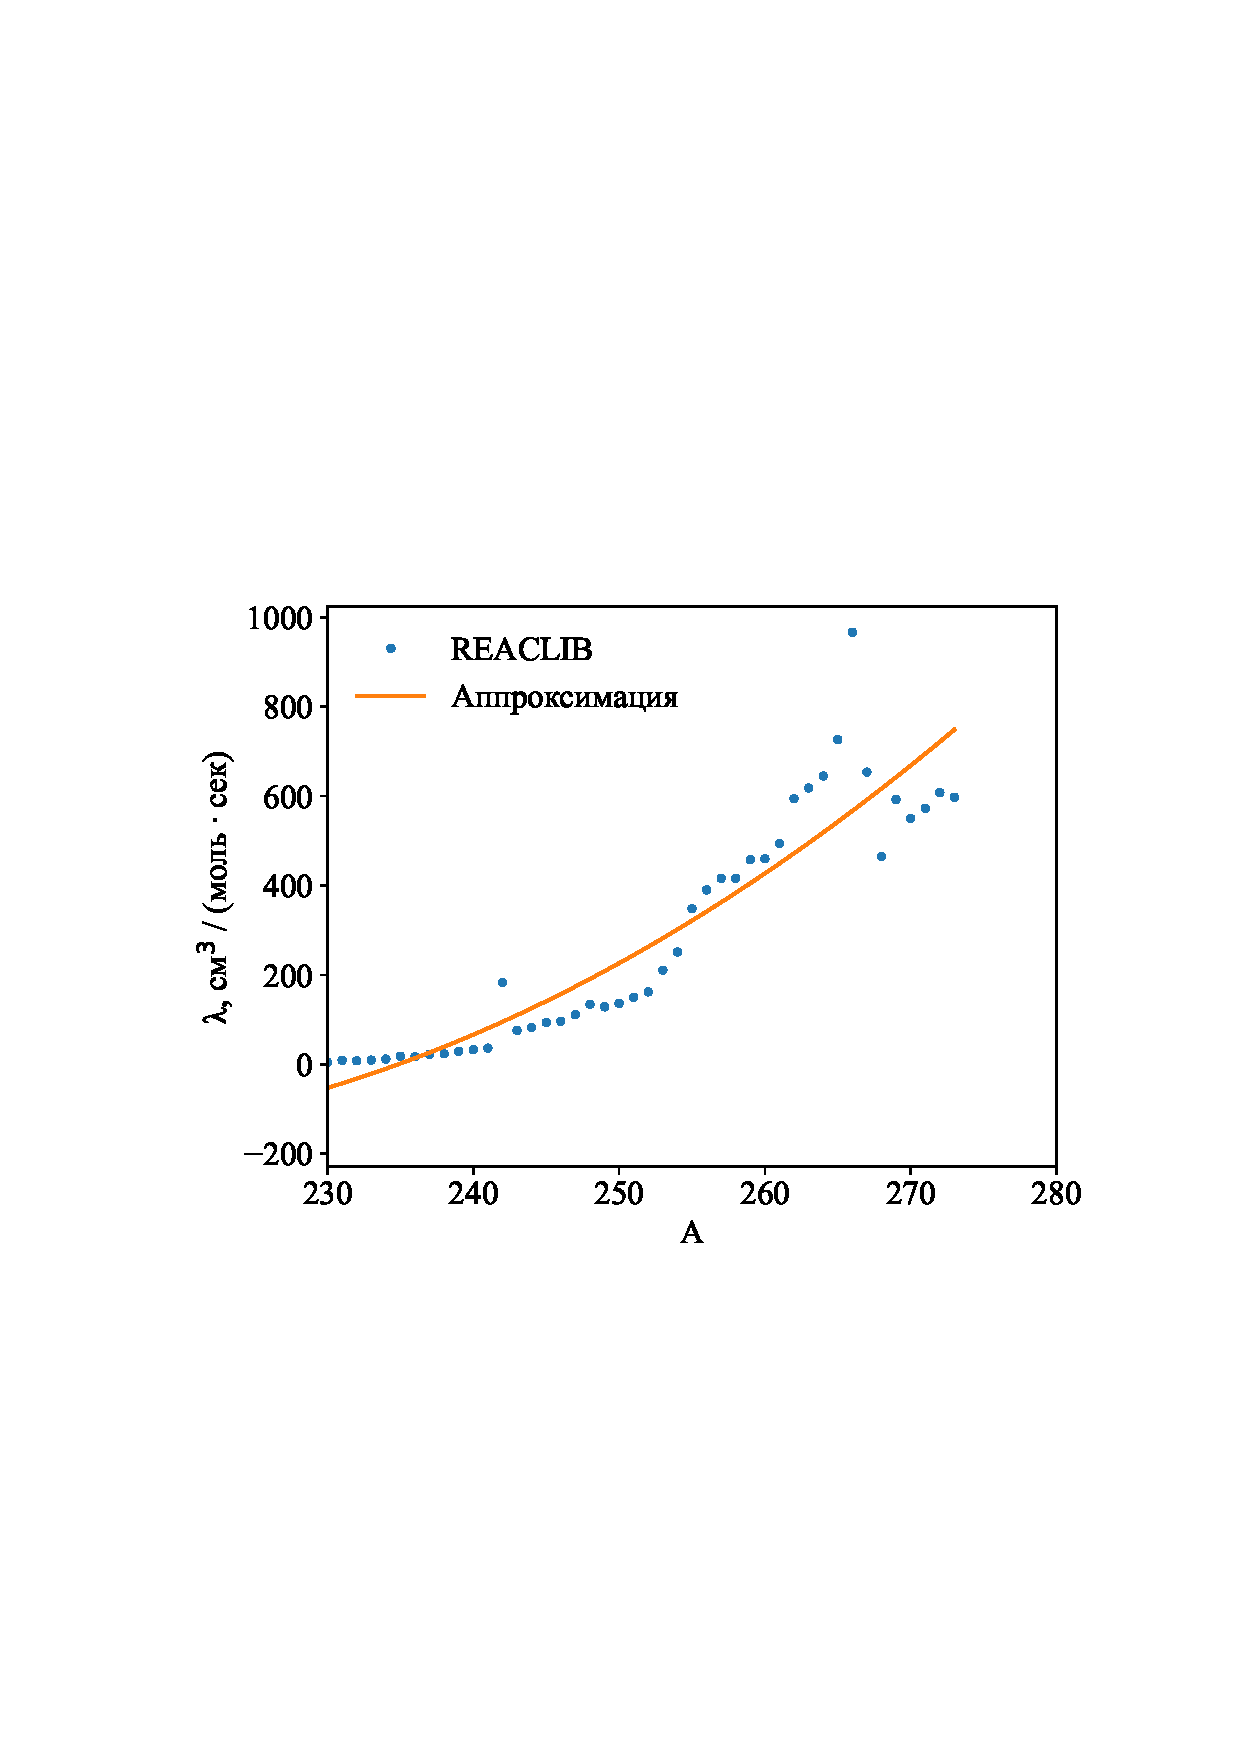
\includegraphics[width=\textwidth]{../pics/decay_fit82.pdf}
    \end{minipage}
    
    Модельная функция --- правило Сарджента: $\lambda_\beta \sim Q_\beta^5$
  }
  
  \frame{
    \frametitle{Астрофизические параметры модели}
    \begin{itemize}
      \item Чаще всего рассматривают сценарий NSM
      \item Начальные условия
      \item Вычисление начальной композиции и плотности
      \item Как меняется плотность в симуляции
      \item Как меняются остальные параметры
    \end{itemize}
  }
  
  \frame{
    \frametitle{Эволюция выходов $r$-изотопов}
    \begin{itemize}
      \item Анимация
      \item Что означает тонкая линия и ее исчезновение
      \item HFB запаздывает!
    \end{itemize}
  }

  \frame{
    \frametitle{Итоговое массовое распределение}
    \begin{itemize}
      \item График распределения
      \item Про неопределенности
      \item Про положение пиков
    \end{itemize}
  }

  \usebeamertemplate{endpage}

  \frame{
    \frametitle{Appendix\\Нейтронный захват за границей существования}
    Просто рис. 7 из диплома и пояснение: мы учитываем реакции даже при $B_n < 0$. C одной стороны, так можно по инерции выходить за пределы границ существования ядер, но, с другой, ничего страшного при этом не происходит, так как скорости там резко падают.
  }

  \frame{
    \frametitle{Appendix\\Слабые распады в библиотеке REACLIB}
    \begin{itemize}
      \item График рис. 9: с какого-то $A$ доминируют распады с вылетом нейтронов.
      \item Мы считаем, что их можно добавлять в скорости $\beta$-распадов при фитировании, потому что недостаток нейтронов быстро компенсируется захватами.
    \end{itemize}
  }
  
  \frame{
    \frametitle{Appendix\\Влияние массовой модели на температуру}
    \begin{itemize}
      \item График рис. 15 
      \item Вроде бы, разница очень маленькая, но
      \item Источник тепла -- $\beta$-распады, а у нас три симуляции различаются в этом плане очень слабо, по границе отделения нейтронов
    \end{itemize}
  }
\end{document}
